\documentclass[10pt,twocolumn]{article}
\usepackage[margin=0.7in,columnsep=0.25in]{geometry}
\usepackage{amsmath,amssymb,booktabs,graphicx,hyperref}
\setlength{\emergencystretch}{1em}
\setcounter{dbltopnumber}{4}
\renewcommand{\dbltopfraction}{0.95}
\renewcommand{\textfraction}{0.05}
\newcommand{\pending}{\textemdash}
\newif\ifFinalReportReady
\IfFileExists{final-results/provenance.tex}{% TEST508: 508 assets, 134 source clusters, five frozen physical pipelines.
% The complete ten-metric, Main, qualitative, and manuscript-input bundles
% have actual file4 SHA256/size PASS closures. This flag enables the
% result-dependent sections; final PDF visual review is a separate gate.
\FinalReportReadytrue
}{}
\title{Ray-Based Semantic Evidence Retargeting for Multi-View 3D Editing}
\author{Anonymous manuscript}
\date{}
\begin{document}
\raggedbottom
\maketitle
\ifFinalReportReady\else
\noindent\textbf{Evaluation-in-progress preview.} The architecture and evaluation
protocol are frozen. Development tables below contain actual measurements;
the final TEST508 table, qualitative panels, and result-dependent writing
remain pending. This preview is not a completed paper.
\fi

\begin{abstract}
An edited image and undeformed source views describe different geometric
states of the same object. Direct multi-view projection can therefore deliver
appearance features to an incorrect region after deformation. We study a
feature retargeting path that retains the native target conditioning and
adapts source evidence through camera-ray groups. A frozen semantic matcher
provides correspondence proposals; the geometry stage shares their weighted
evidence across each ray and uses a gated source-contrast retargeter. The
appearance stage uses a separately evaluated Top-1 retargeter on generated
geometry. We distinguish retrieval diagnostics, matched geometric ablations,
and fixed-geometry appearance comparisons, preserving the pretrained function
at initialization. The evaluation separates source appearance, target
alignment, and global image-distribution endpoints, with source-cluster
uncertainty and a development-only model freeze.
\ifFinalReportReady
On 508 held-out edits from 134 source clusters, the frozen selected pipeline
improves vanilla fine-tuning in source LPIPS ($-0.00104$), target PSNR
($+0.192$ dB), SSIM ($+0.00116$), and mask IoU ($+0.0120$); all four
predeclared 16-endpoint family-adjusted intervals exclude zero. Surface CD
and F-Score have favorable point estimates but unresolved intervals, while
DreamSim and CLIP do not establish a preservation gain. None of the eight
adjusted selected-versus-Top-1-retargeting intervals excludes zero. Thus the
held-out evidence supports specific improvements over vanilla fine-tuning,
while leaving the extra contribution of the selected matching and aggregation
path unresolved.

\else
The completed development studies motivate this stage-specific composition;
the frozen held-out comparison is still running and its findings are not
asserted here.
\fi
\end{abstract}

\begin{figure*}[t]
\centering
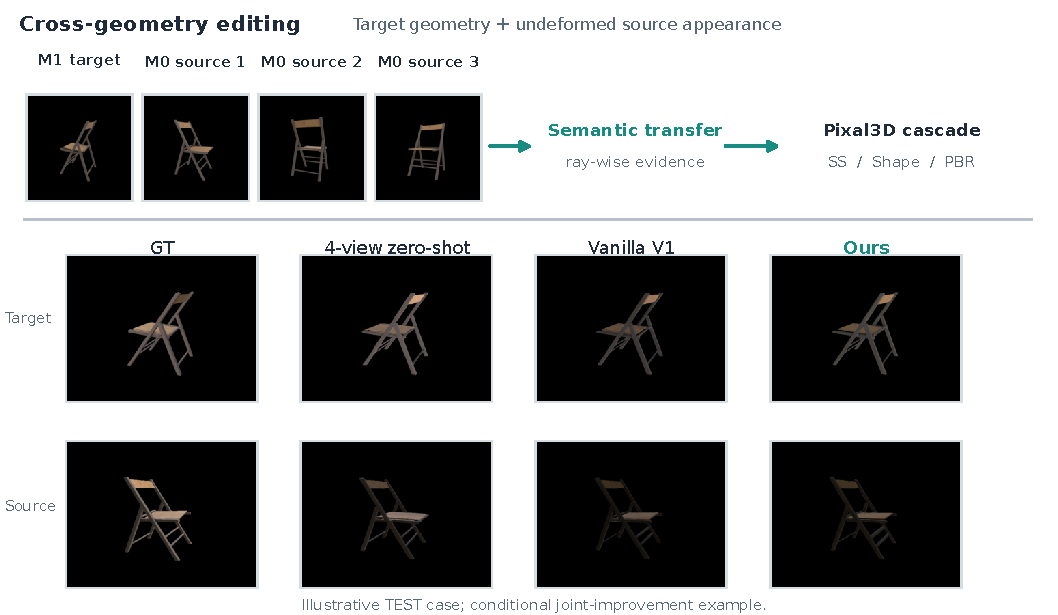
\includegraphics[width=\textwidth]{final-results/figures/paper-teaser.pdf}
\caption{Cross-geometry editing from one edited target RGB view and three undeformed source RGB views. The lower rows compare scored TEST renders at the target camera and one source camera with the common original-material M1 reference. This is the predeclared conditional joint-improvement example, shown to explain the task rather than estimate a population success rate. All compared renders use the archived full-frame pixels and identical cameras.}
\label{fig:teaser}
\end{figure*}

\section{Introduction}
Consider editing an object's shape from a single target image while retaining
appearance evidence from its original views. The edited target and the
sources depict different geometric states. Even with calibrated cameras, a
source feature projected along its original ray need not describe the desired
edited region. A pretrained multi-view generator supplies a useful 3D prior,
but its native spatial associations do not resolve this intentional conflict.

Semantic correspondence can reconnect related regions across the edit.
However, selecting one match can discard a useful alternative, while mixing
many matches can transfer irrelevant values. A better retrieval score also
does not establish that the generated surface or material improves. The
delivery path matters: adapted evidence enters an existing projection-based
conditioning function whose target contribution and source features already
have a trained numerical scale.
Figure~\ref{fig:teaser} illustrates the distinct target and source evidence
and the evaluated view roles.

For paired supervision, we construct DeformNeXt-10k using donor-guided
GeoStyle deformation with source assembly constraints and final-pair
screening. The dataset retains exact canonical mesh correspondence while
providing 10,165 accepted edits from 3,483 source assets, rather than one
fixed edit per object. Section~\ref{sec:data-construction} describes the
construction, split boundary, and limitations of its shortened production
optimization budget.

We study source adaptation within that native function. Voxels projecting to
the same source-camera patch share one evidence decision. A frozen matcher
constructs semantic proposals from the observed target members of that ray;
the selected SS design aggregates native values without a new value/output
projection. A source-contrast retargeter then supplies a gated correction to
the native carrier. Its zero initialization preserves the original function,
and rays without proposal support retain the pretrained prior. The target
conditioning stream is retained; exact target output preservation remains
an evaluation question.

Our experiments distinguish stage objectives. SS candidates are evaluated
for geometric alignment under common frozen downstream models. PBR
candidates are evaluated for source appearance on identical generated
geometry, guides, noise, and rendering triangles. This produces a measured
composition of Fixed Top-K SS and a separate Top-1 retargeting PBR stage,
rather than requiring one aggregation operator to be best at both tasks.

The contributions are an explicit ray-shared source-adaptation formulation;
matched tests separating raw retrieval, decoder descriptors, scalar scores,
aggregation, and retargeting; and a stage-specific evaluation with a frozen
held-out protocol. Candidate coverage, component effects, and final pipeline
quality are separate claims. We retain negative results and uncertainty
instead of inferring necessity from the architecture alone.

\section{Related work}
\paragraph{Generation and editing.}
Sparse representations support high-resolution geometry and materials in
TRELLIS.2~\cite{xiang2025trellis2}; Pixal3D introduces pixel-aligned projection
conditioning~\cite{li2026pixal3d}. Reconstruction--generation combinations
include ReconViaGen~\cite{chang2025reconviagen}, RecGen3D~\cite{huang2026recgen3d},
and GenRecon~\cite{schmid2026genrecon}. We continue the supplied multi-view
LoRA implementation rather than claim projection or multi-view conditioning
as a new mechanism. Its TRELLIS.2/DINOv3 implementation differs from the
published Pixal3D backbone; checkpoint lineage is specified below.

ShapeUP learns source-shape/edited-image translation and uses source renders
for texture~\cite{gat2026shapeup}. GeoStyle deforms a source mesh from an image
style reference~\cite{choi2026geostyle}; APAP~\cite{yoo2024apap} and
SpaceControl~\cite{fedele2025spacecontrol} combine geometric control with
generative priors. TextureDreamer transfers appearance to a supplied target
shape~\cite{yeh2024texturedreamer}. Our evaluated input is instead edited
target RGB plus undeformed source RGB with calibrated cameras, and the output
geometry is predicted. Source-view appearance conditioning itself is not our
novelty claim, and these input differences preclude an unexecuted quantitative
comparison with source-mesh or target-shape methods.

\paragraph{Correspondence and aggregation.}
MV-Adapter supports multi-view generation~\cite{huang2025mvadapter}.
MVDiffusion exchanges correspondence-conditioned information and uses
zero-initialized residual layers~\cite{tang2023mvdiffusion}; this initialization
principle is a safeguard we reuse. CorrAdapter aggregates matched regions
for multi-image consistency~\cite{zhang2026corradapter}. Our question concerns
semantic evidence delivered into a 3D projection-conditioning path when the
observed images intentionally depict different geometries.

Diffusion and DINO features expose complementary correspondence
properties~\cite{tang2023dift,zhang2023twofeatures}. VGGT-$\Omega$
learns geometry-aware representations~\cite{wang2026vggtomega}, and
RoMa-$\Omega$ separates feature similarity, learned probes, and dense
matching~\cite{nordstrom2026romaomega}. Its co-visibility confidence is distinct
from our categorical weighting over retained proposals. These works motivate
separating descriptor quality, matching, aggregation, and generative effects;
they do not establish those effects in our editing task.

\section{Method}
\begin{figure*}[t]
\centering
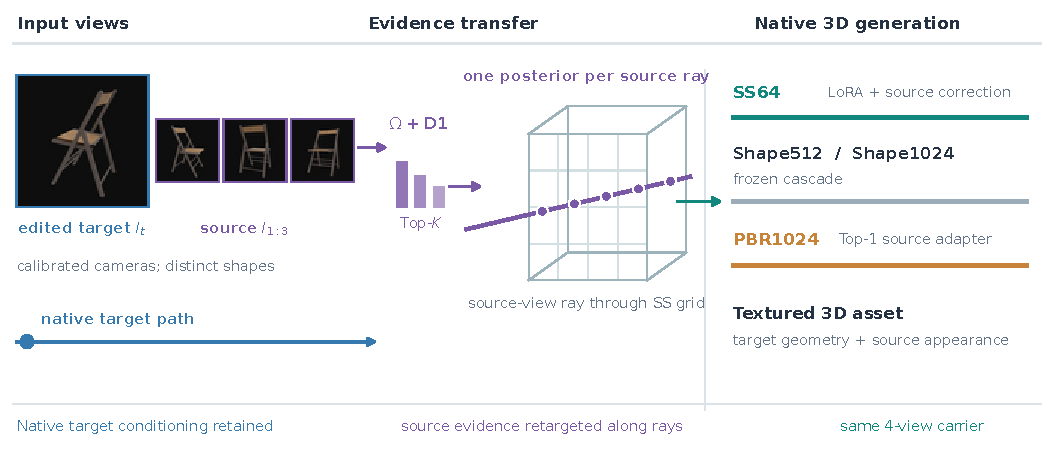
\includegraphics[width=\textwidth]{final-results/figures/paper-overall.pdf}
\caption{Stage-level overview. The edited target follows the native Pixal3D
conditioning path. Semantic evidence from undeformed source views corrects
the SS geometry carrier; Shape512/1024 are frozen. PBR uses a separately
selected Top-1 source retargeter for appearance. Figures~\ref{fig:matching}
and~\ref{fig:retargeting} explain the correspondence and source correction.}
\label{fig:selected-pipeline}
\end{figure*}

\subsection{Native carrier and the sharing unit}
Let $T$ be the target feature map, $S_j$ a source map, and $P_j$ its calibrated
bilinear projection. We retain the native four-view carrier
$C_{\mathrm{MV4}}$, including its target contribution and global tokens.
For source camera $j$ and image patch $p$, the sharing unit is
\begin{equation}
 \mathcal R_{j,p}=\{x:\pi_j(x)=p\}.
\end{equation}
Grid sites on this camera ray share an image-space evidence decision. The
decision is not an independently learned attention output for each voxel
feature. The SS implementation uses a $16^3$ conditioning grid and a
$32\times32$ patch map; SS64 denotes decoded occupancy resolution. Camera
projection defines membership without target surface depth or a
surface-visibility write mask at inference.

\subsection{Semantic proposals and matching scores}
\begin{figure}[t]
\centering
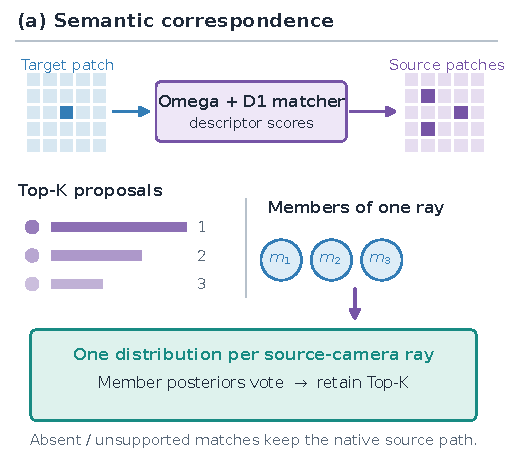
\includegraphics[width=\columnwidth]{final-results/figures/paper-matching.pdf}
\caption{Frozen semantic correspondence. Omega descriptors generate source
proposals and the D1 decoder scores them. Distinct observed target patches
sharing a source-camera ray vote into one Top-K posterior. Matching keys are
separate from the native source values used for generation.}
\label{fig:matching}
\end{figure}
Each observed target patch $m$ retrieves 64 semantic proposals across the
three source images. A frozen D1 decoder contextualizes its descriptor and
produces scores $s_{mk}$. The decoder has one query-only cross-attention block
and a bounded scalar residual head. Matching keys are 1024-dimensional
layer-12 FRAME Omega descriptors; SS values are separate, 1024-dimensional
native DINOv3 features.

Topology-derived barycentric correspondence and training-only depth checks
provide valid positive patch IDs $\mathcal P_m$. Given raw proposals
$\mathcal C_m$, the decoder minimizes
\begin{equation}
 \ell_m=-\log\frac{\sum_{k\in\mathcal C_m\cap\mathcal P_m}e^{s_{mk}}}
                       {\sum_{k\in\mathcal C_m}e^{s_{mk}}}.
\end{equation}
Only queries with a positive proposal contribute. Proposal misses and
unobservable queries are recorded separately. Decoder training uses 9,143
certified training examples and seven passes; Omega and the complete matcher
are frozen during subsequent generative fine-tuning. Topology/depth labels
are supervision and scoring data, not inference conditioning.

Distinct observed target patches in a source ray form its member set
$\mathcal M_r$. Their normalized distributions vote once per member:
\begin{align}
 \bar p_r(k)&=|\mathcal M_r|^{-1}\sum_{m\in\mathcal M_r}p_m(k),\\
 \mathcal K_r&=\operatorname{Top64}(\bar p_r),\qquad
 p_r(k)=\frac{\bar p_r(k)}{\sum_{l\in\mathcal K_r}\bar p_r(l)}.
\end{align}
Missing member entries have zero mass. Scores use softmax temperature 0.05.
This retains complementary modes before truncation instead of matching one
averaged descriptor. Input alpha and camera addresses define observation
support; they are not surface co-visibility. Empty members or insufficient
valid proposals abstain. A concentrated $p_r$ need not be correct: native
fallback detects missing support, not every confident mismatch.

\subsection{Matching-aware aggregation and retargeting}
\begin{figure}[t]
\centering
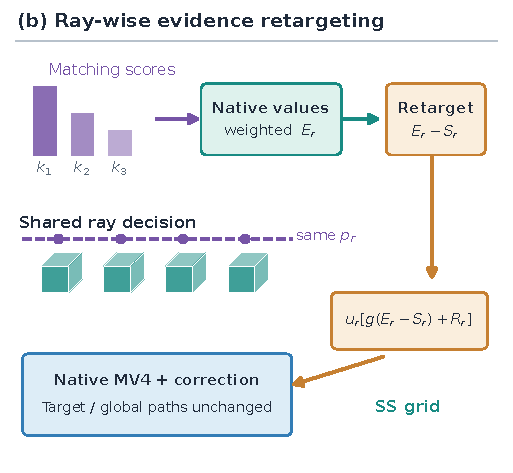
\includegraphics[width=\columnwidth]{final-results/figures/paper-retargeting.pdf}
\caption{One source-camera ray shares its posterior across intersected grid
sites. The selected SS path weights native source values, forms a bounded
source-contrast correction, and adds that correction to the native MV4
carrier. The target contribution and global tokens remain in the carrier;
unsupported rays retain the native source path.}
\label{fig:retargeting}
\end{figure}
The selected SS stage aggregates untransformed native values,
\begin{equation}
 E_r=\sum_{k\in\mathcal K_r}p_r(k)v_k.
\end{equation}
Carrier correction, source use, and retargeting consume this same evidence.
No additional learned Q/K or V/output head is required by this instantiated
design. Such heads are evaluated as alternatives, not declared necessary.

With learned source-use probability $u_r$ and signed bounded gate $g$,
\begin{align}
 R_r&=R_\phi([E_r-S_r,T_r]),\\
 \Delta_r&=u_r\{g(E_r-S_r)+R_r\},\\
 C&=C_{\mathrm{MV4}}+\tfrac14\sum_{j=1}^{3}P_j(\Delta_j).
\end{align}
$T_r$ pools native target context over the ray's grid sites; the distinct
observed members construct the matching distribution. Subtracting $S_r$
accounts for its existing contribution to the carrier. Initially $g=0$ and
the retargeter output is zero, recovering native conditioning. Unsupported
rays retain native source features rather than receive invented zero-valued
observations. Target feature extraction and its direct conditioning path are
retained, but exact generated target RGB preservation is not guaranteed.

\subsection{Stage-specific composition}
SS64 and PBR1024 continue their supplied multi-view LoRA checkpoints;
Shape512/1024 stay frozen. SS uses the weighted Fixed evidence above. The
selected appearance stage uses its separate Top-1 retargeter on generated
geometry. Its values are native DINOv3/NAF features. Neither the PBR feature
variants nor the SS learned-refinement variants are silently substituted for
this selected composition. Stage choices are based on their respective
geometric and fixed-geometry appearance development comparisons.

\section{Experimental setup}
\subsection{DeformNeXt-10k construction}
\label{sec:data-construction}
We construct paired shape edits from the textured assets and hierarchical
part annotations of PartNeXt~\cite{wang2025partnext}. A canonical source
$M_0=(V_0,F,\mathcal A_0)$ defines vertex indices, ordered faces, and the
UV/material/corner-attribute authority. Each accepted variant is
$M_{1,k}=(V_{1,k},F,\mathcal A_0)$: positions change while correspondence
and face connectivity/order remain fixed. Shared face indices and barycentric
coordinates therefore identify corresponding source and edited surface
points without nearest-neighbor reassignment.

\paragraph{Donor-guided proposals.}
We select donors from the same category using frozen semantic-role and
structural-compatibility heuristics. Semantic roles can contain multiple
disconnected pieces; matching individual leaf meshes or requiring equal
part counts would unnecessarily restrict shape diversity. Source/donor
identities and configuration hashes are recorded before each run. Eight
original-appearance donor renders personalize an SDXL prior with
GeoStyle~\cite{choi2026geostyle}. The donor is a morphology prior, rather
than target geometry or an input to the retargeting model.

GeoStyle proposes face-Jacobian changes under image-space score distillation.
Our production path adds a category prompt and source assembly constraints
to the reconstruction: selected primary surfaces deform, complementary
physical components follow rigid motions, and source-derived attachment
proxies couple their movement. These contacts are geometric estimates,
not annotated physical joints. The main production configuration uses
800 donor-specific LoRA updates and 300 deformation iterations; donor LoRA
and source preprocessing are reused across pairs. This shortened configuration
was adopted for throughput and is not demonstrated equivalent to the
official 3,600-iteration configuration. Supplementary details give the
other changes and retained early configurations.

\paragraph{Final-pair selection.}
The category-prompt/assembly proposal (PA) and an optional 120-iteration
Jacobian, crease-aware normal, and neighboring-displacement refinement
(balanced JN-L) are separate candidates. Each is assessed anew against
$M_0$. Agreement with the initial proposal or the donor is not an admission
criterion. We check canonical correspondence, finite geometry and
catastrophic failures, meaningful deformation, paired RGB usability,
native-representation survival, and actual training-loader compatibility.
Multi-view model-assisted screening identifies obvious spikes, detached
components and assembly collapse; it is not independent human validation.
Small intersections, gaps and folds are recorded as diagnostics rather
than universally rejected. The dataset is therefore not certified
intersection-free. Both meshes retain one source-defined 0.48 frame and
are rendered with the source materials and matched cameras; edited meshes
are not independently normalized. All approved distinct variants are
retained, with near-identical final geometries merged.

\begin{figure*}[t]
\centering
\includegraphics[width=\textwidth]{figures/deformnext-construction.pdf}
\caption{DeformNeXt construction and approved source/edited pairs. Donor
images guide morphology; source assembly constrains reconstruction, and each
final candidate is screened independently. Examples show archived RGB
(camera 8) and clay (camera 14), with a common foreground-union display crop
and scale for M0/M1 at each camera. Four categories are drawn from a pre-existing
large-edit illustration selection whose membership was checked against the
final snapshot. They illustrate visible changes, not typical quality,
generator yield or a 300-versus-3,600-step comparison.}
\label{fig:deformnext-construction}
\end{figure*}

\paragraph{Scope and splits.}
The final snapshot contains 10,165 distinct deformations from 3,483 source
UIDs across 50 categories, averaging 2.92 variants per source. This is a
deformation count, not 10,000 independent source objects or an estimate of
yield over all PartNeXt assets. After construction, a fixed seed assigns
approximately 90/5/5 of the examples to train/validation/test while keeping
every source UID and source geometry cluster in one split
(Table~\ref{tab:deformnext-splits}). Donor disjointness is not enforced;
the held-out evaluation measures retargeting on admitted edits from this
construction process, not generalization to an unseen deformation generator.

\begin{table}[t]
\centering
\small
\caption{Frozen DeformNeXt splits. Variants of one source and geometry
cluster stay together; category proportions are not forced to be uniform.}
\label{tab:deformnext-splits}
\begin{tabular}{lrrrr}
\toprule
Split & Edits & UIDs & Clusters & Classes \\
\midrule
Train & 9,149 & 3,184 & 1,790 & 50 \\
Validation & 508 & 153 & 132 & 42 \\
Test & 508 & 146 & 134 & 42 \\
\midrule
Total & 10,165 & 3,483 & 2,056 & 50 \\
\bottomrule
\end{tabular}
\end{table}


\subsection{Training and internal oracle-scale evaluation}
\paragraph{Data and initialization.}
We use the frozen splits in Table~\ref{tab:deformnext-splits}.
PBR training excludes ten recorded oversized training examples,
using 9,139; no test asset is excluded by that training limit. Source UID and
source-asset clusters are disjoint across these deformation splits. Overlap
with earlier multi-view pretraining is not established. The earlier mixed385
subset of 80,892 training and 950 validation assets is pretraining lineage,
not the deformation fine-tuning set.

We load the original configurations and complete base+LoRA weights:
SS64/Shape512 step 4,210 and Shape1024/PBR1024 step 16,850. The matching backbone
is VGGT-Omega epoch 7. SS uses 480 updates, global batch 96, LoRA rank/alpha 16,
and denoiser/conditioner learning rates $10^{-5}/10^{-4}$. PBR uses 1,900
updates, global batch 24, and rates $5\times10^{-6}/10^{-4}$. These are
approximately five training passes. Ablations retain paired inputs,
initialization, budget, sampler, and noise. Removed modules/channels are
physically absent, not filled with zeros.

\paragraph{Development and freeze.}
SS diagnostics use DEV128/93 sources and three paired generation noises,
averaged within an example. Surface ablations use the same 128 examples,
one noise, frozen Shape and common Top-1 R PBR. PBR appearance uses DEV32
with identical generated geometry, archived guides, texture noise, actual
rendering triangles, and references. SS selection uses CD/F-Score; PBR
selection uses source LPIPS/DreamSim with complementary CLIP. Cross-SS
appearance is a secondary diagnostic, not a veto of geometric improvement.

Two independent SS training seeds for V1/R/Fixed and two PBR seeds for
vanilla/R are reported separately. The SS confirmation concerns occupancy;
PBR confirmation is a four-example GT-shape target-camera training diagnostic.
Neither is two-seed full-pipeline quality confirmation. Two fresh loads on
VAL36 verify the selected SS checkpoint, archived latent/occupancy arrays,
prefix32, and the final batch of four. Actual weight/config/cache bindings
and the complete evaluation protocol are frozen before TEST inference.

\paragraph{Comparators and generation.}
The earlier internal oracle-scale TEST comparison contains five physical pipelines: original
source-only RGB4; original edited-target RGB1+source RGB3; vanilla V1;
Top-1 R; and selected Fixed SS+Top-1 R PBR. Source-only includes the original
M0 view at target camera8, not just three sources. Edited inputs are M1 RGB
at8 plus M0 RGB at9/10/11. Shape weights are common. Original zero controls
retain original PBR; V1 uses vanilla 1900 PBR and R/selected use Top-1 R 1900.
SS generation uses batch 8, 12 steps, guidance 3 and the prescribed per-asset
noise map. Native downstream sampling configurations are retained.

Table~\ref{tab:final-main} also includes a post-hoc descriptive input
reference: the original Pixal3D single-view SS, Shape512, Shape1024, and PBR
denoiser checkpoints, with the project's calibrated projective DINO
conditioner, receive only the edited M1 target RGB at camera 8. This is a
project-specific 1024-cascade evaluation, not the official Pixal3D inference
stack. It uses the same 508 TEST examples, per-asset seeds, scoring cameras,
native renderer, and original-material M1 references as the five-model
comparison. The pretrained single-view weights retain their 12-step sampler
defaults, including SS guidance 7.5. There is no multi-view or deformation
fine-tuning. It was evaluated after the five-model freeze, so it is not
included in the adjusted comparison family.

\paragraph{Metrics and references.}
Source LPIPS~\cite{zhang2018lpips}, DreamSim~\cite{fu2023dreamsim}, and separate
OpenAI CLIP image cosine~\cite{radford2021clip} average cameras 9/10. Target
PSNR/SSIM~\cite{wang2004ssim}/2D mask IoU use 8. References use original
materials on edited M1 geometry, not undeformed source pixels. Surface CD
is the symmetric mean unsquared Euclidean nearest-point distance, using
20,000 area-weighted samples. F-Score uses threshold 0.02 in the common
source-defined normalized frame~\cite{tatarchenko2019surface}; there is no
per-output ICP alignment. Voxel IoU is diagnostic. Full-frame image scores
are primary; foreground/GT-only crops are supplementary.

FID~\cite{heusel2017fid}/KID~\cite{binkowski2018kid} use the same 1,524 images
per model/reference, cameras 8--10, official Inception 2048 FP32 features,
and torch-fidelity 0.3.0 float64 reductions. KID uses 100 subsets of 1,000 and
seed 42017, retaining signed raw values. Distribution differences are
descriptive; subset variability is not a source-cluster interval. These are
camera-8/9/10 evaluations, not evidence of general novel-view performance.
The RGB1 reference sees only camera 8, so cameras 9/10 are held out for that
row; the four-view pipelines receive all three scoring cameras as inputs.
This internal table uses the project's native mesh renderer and
black-background image compositing. Its scores are not directly comparable
to the unified Blender/Cycles benchmark below; in particular, the
object-specific M1-derived scale is available at generation only here.

GT raster quality control uses one-pixel edge tolerance and a uniform
whole-pixel rounding of its 1\% allowance. The post-TEST correction and
GT-only audit are disclosed in the Supplement; metric formulas are unchanged.

\paragraph{Statistical scope.}
Means weight deformation examples equally. Paired bootstrap resamples source
clusters, retaining within-source dependence; equal-source sensitivity is
also retained. The development downstream family is six contrasts across
eight endpoints, with 48,000 draws and 48-comparison Bonferroni intervals.
Its geometry endpoints guide SS interpretation; this family is not reduced
after observing results. Stage IoU has its separate six-contrast family.
The selected TEST model versus V1/R uses 4,000 draws with seed 20261022,
eight pairwise endpoints and a 16-comparison family across 134 sources.
Intervals condition on frozen checkpoints and generation, not a population
of training seeds. A zero-containing interval does not prove equivalence.

% Protocol frozen before the camera-calibrated, scale-unprovided TEST evaluation.
% Result-dependent claims and tables are guarded separately in results.tex.
\subsection{Unified benchmark protocol}
\paragraph{Inputs and camera calibration.}
The task provides an edited target RGB view and three RGB views of the
undeformed source object, together with their camera poses, horizontal fields
of view, and acquisition distances. We do not provide an object-specific
scale computed from either the source or the edited target mesh to a
generator. The official single-view Pixal3D control receives only the edited
target RGB and its camera calibration; its projective pipeline uses the native
unit-scale default when the scale argument is absent. Our frozen V1 and
selected multi-view methods use the same image-only scale estimator, trained
on the training split from RGB/A and camera inputs. We report the actual
inputs used by each external method; methods without a calibrated-camera
interface retain their native inference path.

\paragraph{Common population and outputs.}
We evaluate the frozen TEST508 split, report each method's success count out
of 508, and compute cross-method ranking only on the intersection of
successful cases. The new official RGB1 control and our two multi-view
methods use a 1024 cascade, whereas the previously frozen external Pixal3D
baseline uses its native 1536 cascade and estimated cameras. Each retains its
frozen stage sampling settings, which are reported. We do not force other methods to have the same
triangle count: all raw meshes are sampled with the common 20,000-point
surface protocol and rendered at 512 pixels using the same Blender/Cycles
scene, materials, and camera records. For the official single-view Pixal3D
control and our two multi-view methods, we bake a 2048-pixel texture on a
render-only mesh with a preferred budget of 250,000 faces. If native mesh
cleanup or fast simplification fails, or the baked mesh exceeds
0.01 world units of 99th-percentile nearest-neighbor discrepancy from the
untouched output, we retry at 500,000 and then one million faces;
exceptionally complex meshes may then use two or five million faces under the
same acceptance rule. We record the
actual budget per example. The untouched 1024
output is always used for geometric metrics; this bake does not alter the
generation cascade. At budgets of one million faces or higher, we pre-simplify with
\texttt{fast-simplification} 0.2.0 and preserve that render mesh's topology
during PBR baking; the same rule is used for the official and multi-view
Pixal3D controls. Every baked mesh must pass the same 0.01 world-unit check.
Other methods retain their native textured exports under
the common renderer's one-million-face render-only cap. The official
single-view Pixal3D and
the edited-target multi-view pipelines are labeled separately because their
image inputs differ.

\paragraph{Metrics and optional source-mesh registration.}
Source preservation uses LPIPS, DreamSim, and CLIP cosine on cameras 9 and 10.
Global naturalness uses FID and KID on the same common-success image pool.
Target alignment uses PSNR, SSIM, and foreground mask IoU at camera 8, plus
symmetric unsquared Chamfer distance and F-score at threshold 0.02 on the
surface samples. The surface frame is normalized by the input source object's
center and extent, with no per-output alignment in the raw results. A second,
paired condition applies a similarity transform fitted by trimmed symmetric ICP
to the available undeformed source mesh \emph{after} generation. Registration
never uses the edited target mesh, depth, mask, or rendering, and the aligned
textured outputs are rerendered before image metrics are recomputed. The
source-aligned condition forms the main comparison; paired raw results show
the effect of registration separately for target-camera PSNR, SSIM, and mask
IoU on the exact same success subset. We mark the extra source-mesh input
explicitly. Confidence intervals resample source clusters, retaining all
edited examples from a sampled source together. Neither TEST labels nor TEST
metrics choose a scale estimator, model checkpoint, or ICP hyperparameter.

% Development evidence only; do not treat the small native-render PBR panel as
% the final common Cycles evaluation or promote old M1-scale tables here.
% Evidence: docs/superpowers/reports/2026-10-28-scale-ungiven-VAL31-PBR8-paired.json
\paragraph{Scale-unprovided development gate.}
We first hold the image-only scale estimator and the downstream Shape512,
Shape1024, and vanilla PBR weights fixed while changing only the SS stage.
On 31 source-disjoint validation edits, the V1, Retarget, and Selected
variants obtain CD $0.012610/0.012435/0.012367$ and F@0.02
$0.848527/0.850373/0.853088$, respectively. The paired F-score changes
relative to V1 are $+0.001846$ and $+0.004561$; source-cluster bootstrap
95\% intervals are $[-0.007848,+0.011855]$ and
$[-0.005920,+0.016321]$. The intervals include zero, so this panel does not
establish a geometric gain from either module. Its SS occupancy macro-IoU
is $0.443674/0.444928/0.442446$; stage occupancy and decoded mesh quality
are reported separately.

For appearance isolation, we use the same eight image-scale V1 meshes,
initial PBR noise, and native render references for vanilla and Top-1 R PBR.
Their source-camera LPIPS is $0.070836/0.070935$, and target-camera PSNR is
$24.5466/24.5072$ dB. The paired Top-1-minus-vanilla LPIPS and PSNR
intervals are $[-0.000208,+0.000480]$ and $[-0.1018,+0.0174]$ dB.
This small native-render panel does not establish appearance improvement;
the final Blender/Cycles comparison and source-M0 postprocessing remain
separate evaluations.


\section{Results}
\subsection{Frozen held-out comparison}
\ifFinalReportReady
\begin{table*}[t]
\centering\scriptsize
\resizebox{\textwidth}{!}{%
\begin{tabular}{lrrrrrrrrrr}
\toprule
&\multicolumn{3}{c}{Source preservation}&\multicolumn{2}{c}{Global naturalness}&\multicolumn{5}{c}{Target alignment}\\
Model&LPIPS$\downarrow$&DreamSim$\downarrow$&CLIP$\uparrow$&FID$\downarrow$&KID$\downarrow$&PSNR$\uparrow$&SSIM$\uparrow$&M-IoU$\uparrow$&CD$\downarrow$&F-Score$\uparrow$\\
\midrule
Zero-shot, source-only RGB4&0.061884&0.153975&0.943278&36.089871&0.0014905934&22.4062&0.936489&0.814896&0.0167443&0.766221\\
Zero-shot, edited target + source RGB3&0.058324&0.154276&0.942090&35.024202&0.001618189&23.5416&0.945824&0.882545&0.0148793&0.808255\\
Vanilla V1&0.057245&0.151460&0.942854&34.658819&0.0017537581&23.8360&0.946375&0.889032&0.0141140&0.828473\\
Top-1 R&0.056329&0.151162&0.943177&34.930351&0.001822029&23.9966&0.947295&0.898210&0.0136234&0.834758\\
Selected model&0.056201&0.152069&0.943018&34.361368&0.0016011107&24.0283&0.947532&0.901072&0.0136001&0.834532\\
\bottomrule
\end{tabular}}
\caption{Actual frozen TEST508 results from134 source clusters. Source LPIPS/DreamSim/CLIP average cameras9/10; target PSNR/SSIM/2D mask IoU use camera8. Surface CD is symmetric unsquared Euclidean distance; F-Score uses threshold0.02 in the common normalized frame. Official Inception2048 FID/KID use the same1524-image prediction/reference pools. KID is signed and shown in raw units, without clipping or rescaling. References use original materials on edited M1 geometry. These are input-camera evaluations. The selected physical model is SELECTED; a merged baseline is not repeated as another model.}
\label{tab:final-main}
\end{table*}

Table~\ref{tab:final-main} reports the complete frozen five-pipeline
comparison plus the added single-view reference on 508 TEST objects and 134
source clusters. The added RGB1 row has the highest target input-camera
PSNR/SSIM/mask IoU points (24.543 dB/0.95139/0.92725), but its surface CD
and F-Score (0.01789/0.74311) are worse than the four-view edited zero-shot
and selected models. Its source LPIPS/DreamSim/CLIP are
0.06090/0.16202/0.94062, versus 0.05620/0.15207/0.94302 for the selected
model. Original single-view denoisers and native guidance differ from the
multi-view controls, so these descriptive differences cannot be attributed
to view count alone. Within the frozen five-model family, supplying the edited
target RGB changes the zero-shot target PSNR from 22.406 to 23.542 dB,
mask IoU from 0.8149 to 0.8825, CD from 0.01674 to 0.01488, and surface
F-Score from 0.7662 to 0.8083. Vanilla fine-tuning reaches 23.836 dB,
0.8890, 0.01411, and 0.8285, respectively. These zero-shot and vanilla
comparisons are descriptive; the predeclared adjusted family tests the
selected pipeline against the two fine-tuned controls. The different
zero-shot inputs separate access to edited RGB evidence from the subsequent
fine-tuning comparison, without treating input availability as a learned
module effect.

The selected Fixed-SS/Top-1-R-PBR composition has source LPIPS 0.05620 and
target PSNR 24.028 dB, SSIM 0.94753, and mask IoU 0.90107. Relative to
vanilla V1, the paired differences are $-0.001044$, $+0.1923$ dB,
$+0.001156$, and $+0.012041$. Their 16-endpoint family-adjusted 95\%
intervals exclude zero (Supplementary
Table~\ref{tab:final-adjusted-contrasts}). The selected pipeline has a
lower CD point estimate (0.01360 versus 0.01411) and a higher surface
F-Score (0.83453 versus 0.82847), but the adjusted intervals for both
contain zero. Source DreamSim is 0.15207 versus V1's 0.15146, and its
adjusted interval also contains zero; the same is true for source CLIP.
Thus the held-out support is endpoint-specific, rather than a claim that
geometry and source appearance improve on every measure.

Against the Top-1 retargeting baseline, the selected pipeline has small
favorable points for LPIPS, target PSNR, SSIM, mask IoU, and CD, but a
higher (worse) DreamSim and slightly lower F-Score. Every one of the eight
predeclared adjusted intervals contains zero. This comparison does not
establish that the selected Top-K weighted SS path contributes additional
held-out quality beyond the retargeting baseline, nor does it establish
equivalence. The added single-view baseline has the lowest FID point (34.147),
while the source-only four-view zero-shot model has the lowest KID point
(0.001491). FID
and signed raw KID summarize common 1,524-image input-camera pools and are
descriptive, without a paired significance claim.

\else
The five-model TEST508 cascade and ten-metric evaluation are in progress.
The final Main table will be imported from the closed source-bound collector;
development means are not substituted into it. The comparison separates the
information supplied by an edited target from the effect of fine-tuning and
retargeting. Its geometric and appearance findings remain unasserted here.
\fi

\subsection{Geometric component comparisons}
\input{typeset/final-ablation-template.tex}
All seven SS designs have completed 480 updates, DEV128 three-noise
diagnostics, and actual surface evaluation under common downstream models.
Spatial, raw semantic, decoder-cosine and scalar Fixed give CD 0.0129704,
0.0128789,0.0128065 and 0.0127572, with F-Score 0.839333,0.841031,0.842414
and 0.844058. The point-estimate ladder improves both geometric endpoints,
but every interval in the 48-comparison family includes zero.

Fixed minus Top-1 changes F-Score by 0.003963, with adjusted
interval $[-0.000910,0.009748]$; Fixed minus Uniform gives 0.001553 with
$[-0.003326,0.007439]$; physical retargeter removal gives a Fixed advantage
of 0.009020 with $[-0.001582,0.020293]$. CD intervals also contain zero.
We select Fixed by the lowest CD/highest F-Score points, while retaining
uncertainty about component effects. Spatial 3 versus semantic 64 is a
module substitution, Top-1 versus weighted Top-K bundles candidate count
and aggregation, and scalar matching can change support. Uniform on the
same support is the separate weighting control.

\subsection{Appearance on identical selected geometry}
\input{typeset/dev-selected-pbr-appearance32.tex}
The four PBR variants share actual generated Fixed geometry, native guides,
texture noise, triangles and references. Top-1 R has the lowest source
LPIPS/DreamSim points, 0.053290/0.157828, versus vanilla 0.053513/0.158346.
Their exploratory paired deltas are $-0.000223$ with
$[-0.000539,0.000035]$ and $-0.000517$ with $[-0.002250,0.001183]$.
Both intervals include zero. Feature/Raw variants do not improve either
primary point over Top-1 R; vanilla has the best complementary CLIP point.
We choose the measured Top-1 R PBR and report target image metrics separately.
Identical CD/F-Score confirm geometry equality, not a PBR geometry gain.
The feature/Raw arms retain a Top-1 carrier/use path and do not establish the
effect of a shared Fixed PBR pathway.

\subsection{Retrieval evidence and generated quality}
Decoder matching improves exact rank-one coverage from 1.25\% to 7.73\%
in the separate DEV32 diagnostic. Member proposals raise exact@64 coverage
from 50.76\% to 73.36\%. Native evidence-use analysis finds 31,408 observable
Top-1-miss/Top-K-hit relations; Fixed places more probability on GT proposals
than post-hoc Uniform. These measurements establish available evidence and
its allocation, not a generated-quality improvement. The original learned
ray-versus-voxel and member-versus-mean studies do not establish positive
quality effects; their scope differs from the selected identity-value path.
Full diagnostics and the actual annotated example are in the Supplement.

\subsection{Prespecified qualitative comparison}
\ifFinalReportReady
\begin{figure*}[!t]
\centering
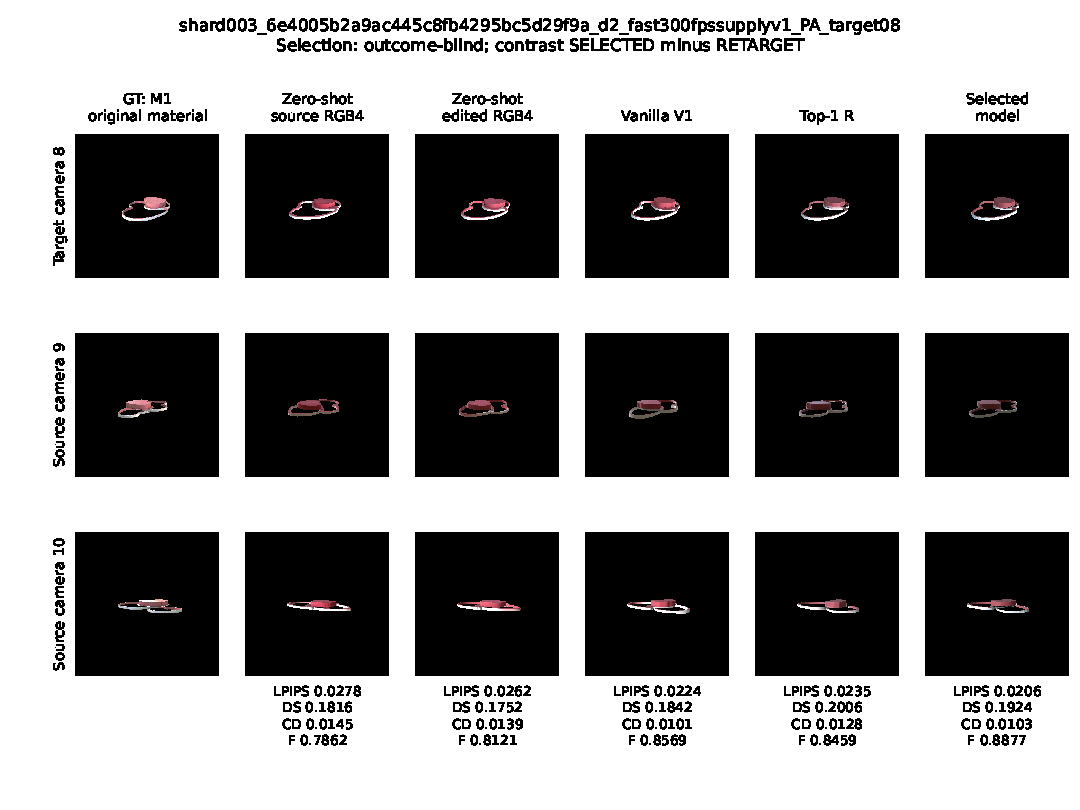
\includegraphics[width=\textwidth]{final-results/figures/example-01.pdf}
\caption{Actual scored frozen TEST example. Rows are target8/source9/source10; columns are the common original-material M1 reference and every frozen model. Selection: outcome-blind. Full-frame panels use the scored archive and official uint8 conversion, without model-specific crop, alignment or rerender. Source annotations use cameras9/10. Conditional categories illustrate their stated conditions and do not estimate population success rates.}
\label{fig:final-qualitative-01}
\end{figure*}

\else
The Main figure is reserved for the first outcome-blind example in the
original metadata declaration. The second outcome-blind example and every
conditional lower-median panel remain in the Supplement. This placement is
fixed before viewing the final panels and is independent of their quality.
The actual scored target/source images will be imported after ten-metric
completion; no placeholder image is presented as an experiment.
\fi

\section{Discussion and limitations}
\ifFinalReportReady
The frozen held-out comparison supports a narrow conclusion: composing the
selected geometry and appearance stages improves source LPIPS and three
target-image endpoints over vanilla V1 under the declared adjusted family.
Surface CD and F-Score remain uncertain despite favorable points. The
selected-versus-Top-1-R comparison is unresolved on every adjusted
endpoint. These results cannot identify semantic matching, matching score,
ray aggregation, or the retargeter as individually necessary. The completed
DEV matched studies also leave their component-level 48-comparison
intervals crossing zero; retrieval coverage and attention allocation are
mechanism evidence rather than generated-quality guarantees.

The outcome-blind panels retain their predetermined samples, while the
conditional Supplement includes joint improvement and separate geometry-
and appearance-loss cases. Those categories expose failures and are not
population success rates. All displayed panels use the scored full-frame
archives and common M1 original-material reference. The native target
conditioning stream remains intact, but the complete generator does not
guarantee pixel-exact target RGB preservation. The PBR selection is a
same-geometry appearance comparison; the evaluated PBR feature/Raw
alternatives use a Top-1 carrier and do not test a shared weighted Top-K
appearance path.

The estimates condition on one frozen full-pipeline checkpoint and one
prescribed generation noise per TEST asset. Two SS training seeds and the
small PBR training diagnostic do not measure full-cascade training-seed
uncertainty. The TEST sources are disjoint within DeformNeXt, but possible
overlap with earlier multi-view pretraining has not been audited. Metrics
use the specified input cameras; they do not establish novel-view editing
quality. FID and KID are renderer-dependent distribution summaries, and
their point differences have no source-cluster interval. Foreground and
GT-crop sensitivity is reported separately without redefining the
full-frame primary endpoints.

\fi
\paragraph{Stage objectives and the delivery path.}
An SS geometric change can alter rendered source appearance even with a
common PBR, so cross-SS LPIPS/DreamSim cannot establish an appearance-module
effect. Conversely, fixed-geometry PBR comparisons do not test geometric
improvement. We report both groups for the composed system while selecting
each stage for its own objective. Native target conditioning is retained,
but the output depends jointly on all stages and need not preserve target
RGB exactly.

\paragraph{Candidate uncertainty.}
Higher candidate coverage and GT probability mass need not improve a
generated asset. A well-supported ray can still match incorrectly; support
is not physical visibility and relative posterior mass is not calibrated
correctness. The native fallback handles absent evidence, not every
confident mismatch. Additional learned refinement has not established a
surface-quality advantage in the completed development comparison. The
existence of ray sharing, semantic matching, or attention does not prove
their necessity.

\paragraph{Scope of the evidence.}
The original FULL, its ray/member controls, and the selected shared-evidence
design differ in multiple components. Their differences do not isolate
shared routing or the final ray unit. Two SS training seeds confirm
occupancy trends of combined branches; the two-seed PBR diagnostic uses
four GT-shape target examples. Neither quantifies full-pipeline training-seed
variability. Test sources are disjoint within DeformNeXt, while overlap with
earlier multi-view pretraining is not audited. Input-camera evaluation and
renderer-specific FID/KID do not establish novel-view quality or human
naturalness judgments. Full-frame appearance scores can be influenced by
background; the existing foreground/GT-crop sensitivity is reported
separately without changing the primary endpoints.


\section{Conclusion}
\ifFinalReportReady
We evaluated semantic evidence retargeting within a frozen multi-view 3D
editing pipeline, selecting SS for geometry and PBR for appearance before
the held-out test. On TEST508, the selected composition improves vanilla
fine-tuning on source LPIPS and target PSNR, SSIM, and mask IoU under the
predeclared adjusted comparison. Surface geometry gains and an additional
benefit over the Top-1 retargeting baseline remain uncertain. The resulting
claim is a measured pipeline-level improvement on specified endpoints,
while the separate necessity of matching, weighting, and ray-based
aggregation remains an open empirical question.

\else
We formulate semantic feature retargeting as source adaptation within a
pretrained multi-view carrier and distinguish the geometric and appearance
objectives of its stages. The completed development ablations provide
conditional evidence and unresolved component-level uncertainty; they do not
establish that every matching or attention component is necessary. The final
conclusion will follow the complete frozen TEST508 comparison.
\fi

\clearpage
\bibliographystyle{plain}
\bibliography{references}
\clearpage
\appendix
\section{Supplementary evidence and reproducibility}
This Supplement retains complete development studies and their limits. It
does not reinterpret exploratory results as held-out confirmation.

\subsection{Architecture, matcher and training details}
D1 has one query-only cross-attention block with four heads of width 32 and
a 128-dimensional feed-forward bottleneck. Candidate descriptors are unchanged.
A LayerNorm--MLP scalar head of hidden width 64 adds a bounded
$0.25\tanh$ residual to contextual cosine. The listwise objective averages
eligible queries within an asset; assets without an eligible query do not
update the matcher. The final seven-pass checkpoint contains 62,545 updates,
using AdamW rate $10^{-4}$, weight decay 0.01 and gradient clipping 1. Six
teacher-rejected cases affect matcher training only; the SS population is
still 9,149. No test matching-head training or calibration is performed.

The selected SS uses identity values and no new learned readout. An evaluated
alternative anchors learned logit refinement to its initial score:
\begin{equation}
 a_{rhk}=\operatorname{softmax}_{k\in\mathcal K_r}
 [\log p_r(k)+s_{rhk}(\theta)-s_{rhk}(\theta_0)].
\end{equation}
Four-head probabilities average before native value aggregation. Prior-weighted
centering of the score difference preserves this softmax, and zero prior
support remains zero. This initialization reproduces Fixed weights, but an
initialization safeguard is not evidence of a quality advantage. Learned
V/output transforms are distinct alternatives. Absent deformation-query
channels and source modules are physically removed in their respective
controls.

The original SS/PBR base and frozen matcher tensors, LoRA initialization,
per-rank input/noise/timestep traces, and saved checkpoint/config hashes are
verified in the experimental artifacts. Main SS comparisons use a native
microbatch 96 without accumulation; native PBR uses four ranks with
microbatch 6, accumulation 1 and global batch 24. Shape stages, image encoders,
Omega and the matching decoder remain frozen during generative fine-tuning.

\subsection{Original module family and independent training}
\input{typeset/dev-ss128.tex}
\input{typeset/dev-original-module-effects.tex}
\input{typeset/dev-independent-ss.tex}
The original 12-model family has ten prespecified module contrasts; its
adjusted intervals include zero. Two follow-up evidence designs are reported
separately. In the original FULL family, ray minus voxel macro IoU is
$-0.000236$, with adjusted interval $[-0.000878,0.000351]$. Member minus mean
is$-0.000601$, with $[-0.002246,0.001262]$. These results do not establish a
positive quality effect or equivalence, and the original learned readout is
not the selected Fixed architecture.

The two-seed SS study uses 4,000 source-cluster draws for three IoU contrasts
separately within each seed and for the fixed-two-checkpoint mean. It is not
a simultaneous nine-comparison or training-seed-population interval. Fixed
minus V1 is positive in both actual runs; Fixed minus Top-1 remains uncertain.
For selected Fixed SS, two fresh VAL36 loads verify latent/occupancy
consistency and tail-batch behavior before TEST. The V1/Top-1 controls retain
their own archived checkpoint-binding and native parity checks; these are
not a two-fresh-load study of all seven ablation checkpoints.

\input{typeset/dev-independent-pbr.tex}
The two-seed PBR training diagnostic retains each producer's fixed-four
GT-shape target reference and declared initial-render policy. Across seeds,
input RGB, cameras, noise and initial latent checks are exact, but these
curves are not pooled as common-pixel source-preservation evidence.

\subsection{Paired geometric and appearance studies}
\input{typeset/dev-geometry-contrasts128.tex}
\input{typeset/dev-completed-fixed-contrasts.tex}
\input{typeset/dev-joint32.tex}
\input{typeset/dev-joint128.tex}
\input{typeset/dev-pbr-appearance32.tex}
\input{typeset/dev-paired-pbr32.tex}
All 48 downstream family values are retained unrounded in the source-bound
artifact. The displayed geometric intervals use that complete correction;
the separate SS diagnostic family averages three noises per asset. The
historical V1-geometry PBR table and the same-selected-Fixed table in the Main
text describe different fixed geometries. Their points are not exchanged or
pooled. Generated-geometry appearance and geometry results remain distinct
from fixed-GT-shape training diagnostics.

\subsection{Matching evidence and its limits}
\input{typeset/dev-matching32.tex}
\input{typeset/dev-ray-evidence.tex}
On 31,408 native observable Top-1-miss/Top-K-hit relations, mean GT mass is
1.6266\% for post-hoc Uniform, 6.4601\% for Fixed, and 6.1756\% for learned
refinement. The learned-minus-Fixed interval includes zero. Candidate
diagnostics and a relationship's stored annotation do not establish a
population quality gain or a visibility calibration. The illustration is
selected by the original conditional lexicographic rule, not downstream
render quality. Post-hoc Uniform mass is not the matched Uniform training arm.

\subsection{Full-frame and foreground sensitivity}
The primary table retains full-frame metrics. The existing producer also
reports foreground PSNR and GT-only-crop DreamSim/CLIP, with common GT-defined
crops across models. These reveal sensitivity to foreground/background
composition without model-specific recentering or alignment. They are
supplementary descriptive endpoints, not a new primary family.
\ifFinalReportReady
\begin{table*}[t]
\centering\scriptsize
\setlength{\tabcolsep}{4pt}
\begin{tabular}{lrrrr}
\toprule
\multicolumn{5}{l}{A. Source appearance: full frame and common GT-defined crop}\\
Model&DreamSim full$\downarrow$&DreamSim crop$\downarrow$&CLIP full$\uparrow$&CLIP crop$\uparrow$\\
\midrule
Zero-shot, source-only RGB4&0.153975&0.184780&0.943278&0.934490\\
Zero-shot, edited target + source RGB3&0.154276&0.186046&0.942090&0.935730\\
Vanilla V1&0.151460&0.184041&0.942854&0.937057\\
Top-1 R&0.151162&0.183377&0.943177&0.936402\\
Selected model&0.152069&0.183833&0.943018&0.935886\\
\midrule
\multicolumn{5}{l}{B. Pixel alignment: full frame and alpha-union foreground}\\
Model&\shortstack{Source PSNR\\full$\uparrow$}&\shortstack{Source PSNR\\foreground$\uparrow$}&\shortstack{Target PSNR\\full$\uparrow$}&\shortstack{Target PSNR\\foreground$\uparrow$}\\
\midrule
Zero-shot, source-only RGB4&23.17341&11.74087&22.40621&10.94126\\
Zero-shot, edited target + source RGB3&23.46619&11.90479&23.54157&11.78260\\
Vanilla V1&23.62321&12.05047&23.83599&12.06429\\
Top-1 R&23.70646&12.11024&23.99656&12.18422\\
Selected model&23.71804&12.11966&24.02827&12.21706\\
\bottomrule
\end{tabular}
\caption{Existing supplementary scores for the complete frozen TEST508 pipelines. Source means use cameras9/10; target means use camera8. Crops use the common GT-alpha bounding box with10\% padding. Foreground PSNR uses the union of predicted/GT alpha$>0.5$ and can have output-specific support. These descriptive composed-pipeline sensitivities do not isolate a PBR effect, change the primary family, or reselect a checkpoint.}
\label{tab:final-foreground}
\end{table*}

\begin{table*}[t]
\centering\scriptsize
\begin{tabular}{llrrl}
\toprule
Contrast&Endpoint&Difference&Family-adjusted95\% interval&Interpretation\\
\midrule
Selected minus Vanilla V1&LPIPS&-0.001044&$[-0.001715,-0.000446]$&benefit supported\\
Selected minus Vanilla V1&DreamSim&0.000609&$[-0.002974,0.003841]$&uncertain\\
Selected minus Vanilla V1&CLIP&0.000164&$[-0.002010,0.002200]$&uncertain\\
Selected minus Vanilla V1&PSNR&0.1923&$[0.0703,0.3201]$&benefit supported\\
Selected minus Vanilla V1&SSIM&0.001156&$[0.000538,0.001833]$&benefit supported\\
Selected minus Vanilla V1&M-IoU&0.012041&$[0.005487,0.021451]$&benefit supported\\
Selected minus Vanilla V1&CD&-0.0005139&$[-0.0014386,0.0000208]$&uncertain\\
Selected minus Vanilla V1&F-Score&0.006059&$[-0.000676,0.013572]$&uncertain\\
Selected minus Top-1 R&LPIPS&-0.000129&$[-0.000530,0.000291]$&uncertain\\
Selected minus Top-1 R&DreamSim&0.000907&$[-0.001656,0.003761]$&uncertain\\
Selected minus Top-1 R&CLIP&-0.000159&$[-0.002212,0.001829]$&uncertain\\
Selected minus Top-1 R&PSNR&0.0317&$[-0.0653,0.1267]$&uncertain\\
Selected minus Top-1 R&SSIM&0.000237&$[-0.000321,0.000673]$&uncertain\\
Selected minus Top-1 R&M-IoU&0.002863&$[-0.000239,0.008191]$&uncertain\\
Selected minus Top-1 R&CD&-0.0000233&$[-0.0001668,0.0000903]$&uncertain\\
Selected minus Top-1 R&F-Score&-0.000226&$[-0.003362,0.002879]$&uncertain\\
\bottomrule
\end{tabular}
\caption{All predeclared selected-versus-control primary comparisons, using the existing source-cluster-adjusted intervals. Source LPIPS/DreamSim/CLIP use9/10; target PSNR/SSIM/M-IoU use8; CD/F-Score use generated surfaces. Values are rounded for display; interpretation uses the original unrounded intervals and metric directions. An interval containing zero does not prove equivalence. FID/KID remain descriptive and are not included in this inferential family.}
\label{tab:final-adjusted-contrasts}
\end{table*}

\else
The actual final foreground table and 16 adjusted primary comparisons are
pending complete frozen ten-metric collection.
\fi

\subsection{Qualitative selection and remaining examples}
The original metadata declaration fixes two examples from distinct sources
without candidate scores. The first is placed in the Main text; the second
and every conditional lower-median example are included here. Empty categories
remain empty and overlapping categories share one panel. Category counts
describe eligibility, not population success rates. Images reuse exactly the
scored float arrays and official uint8 conversion, with target8/source9/10,
common M1 original-material references, and no model-specific crop or rerender.
\ifFinalReportReady
\paragraph{Predeclared conditional eligibility.}
joint-improvement: 77 eligible. The selected lower-median example appears in Fig.~\ref{fig:final-qualitative-03}.
geometry-loss: 191 eligible. The selected lower-median example appears in Fig.~\ref{fig:final-qualitative-04}.
appearance-loss: 153 eligible. The selected lower-median example appears in Fig.~\ref{fig:final-qualitative-05}.
Overlapping conditions share one panel. The first outcome-blind panel stays in the Main text even when it also satisfies a conditional category; it is referenced here rather than duplicated.
\begin{figure*}[!t]
\centering
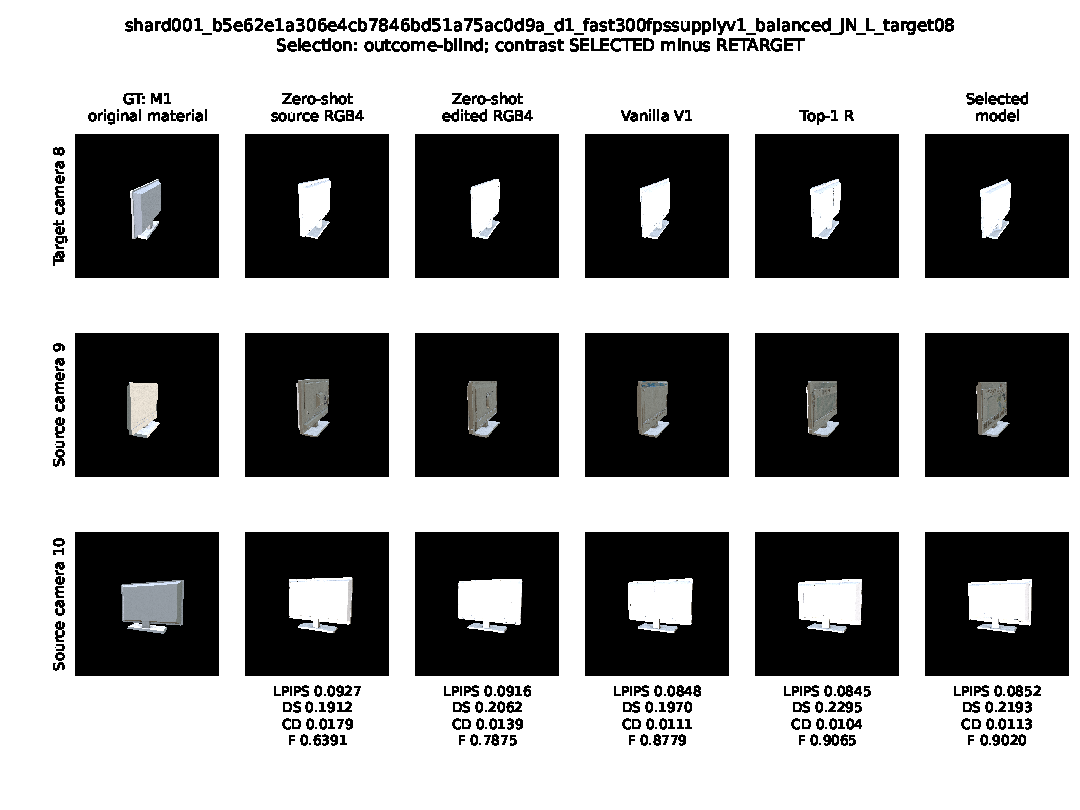
\includegraphics[width=\textwidth]{final-results/figures/example-02.pdf}
\caption{Actual scored frozen TEST example. Rows are target8/source9/source10; columns are the common original-material M1 reference and every frozen model. Selection: outcome-blind. Full-frame panels use the scored archive and official uint8 conversion, without model-specific crop, alignment or rerender. Source annotations use cameras9/10. Conditional categories illustrate their stated conditions and do not estimate population success rates.}
\label{fig:final-qualitative-02}
\end{figure*}
\begin{figure*}[!t]
\centering
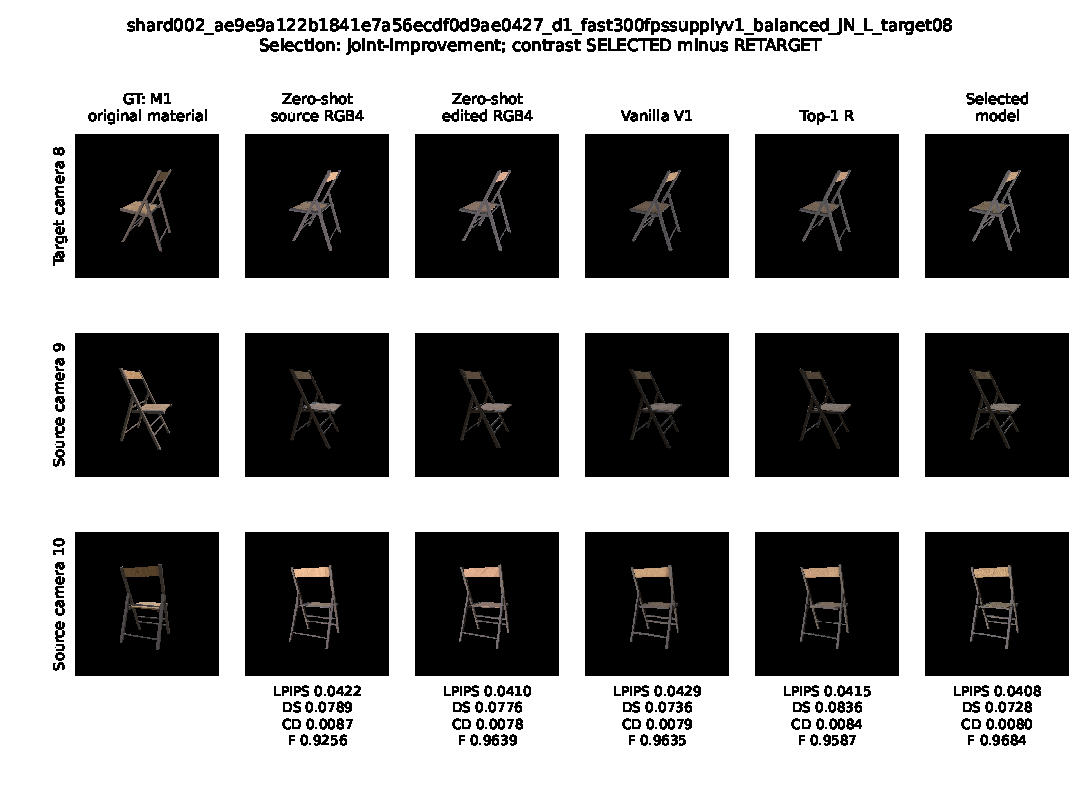
\includegraphics[width=\textwidth]{final-results/figures/example-03.pdf}
\caption{Actual scored frozen TEST example. Rows are target8/source9/source10; columns are the common original-material M1 reference and every frozen model. Selection: joint-improvement. Full-frame panels use the scored archive and official uint8 conversion, without model-specific crop, alignment or rerender. Source annotations use cameras9/10. Conditional categories illustrate their stated conditions and do not estimate population success rates.}
\label{fig:final-qualitative-03}
\end{figure*}
\begin{figure*}[!t]
\centering
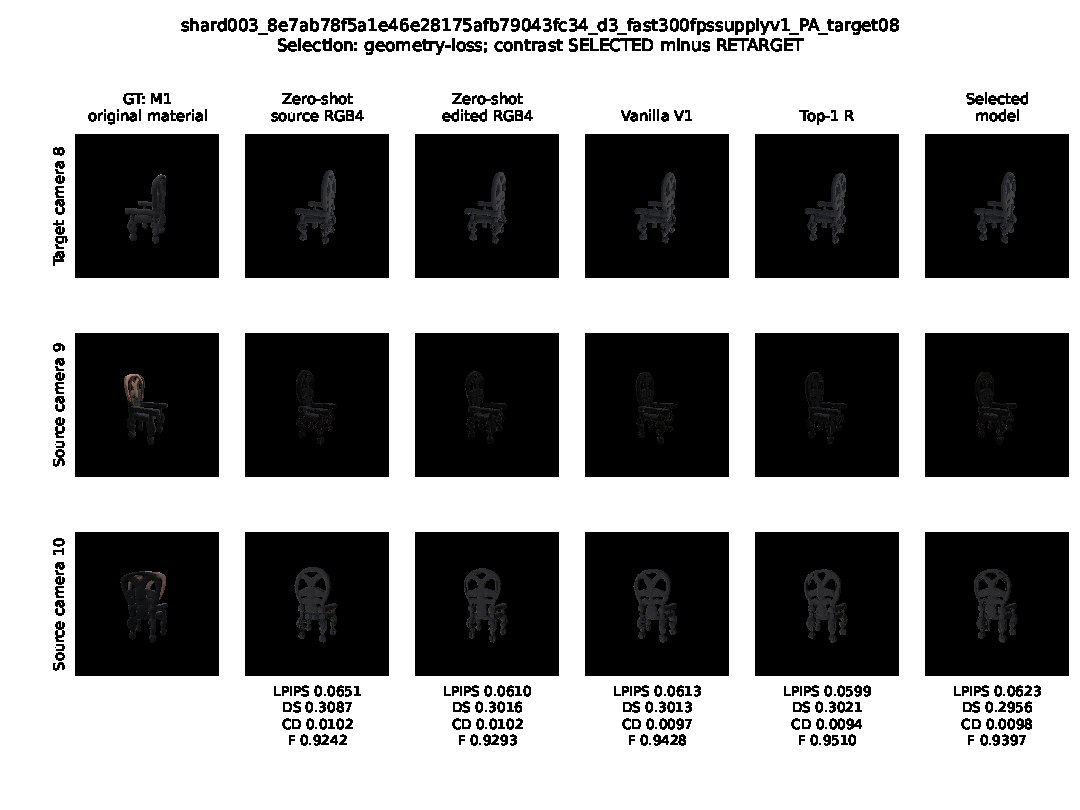
\includegraphics[width=\textwidth]{final-results/figures/example-04.pdf}
\caption{Actual scored frozen TEST example. Rows are target8/source9/source10; columns are the common original-material M1 reference and every frozen model. Selection: geometry-loss. Full-frame panels use the scored archive and official uint8 conversion, without model-specific crop, alignment or rerender. Source annotations use cameras9/10. Conditional categories illustrate their stated conditions and do not estimate population success rates.}
\label{fig:final-qualitative-04}
\end{figure*}
\begin{figure*}[!t]
\centering
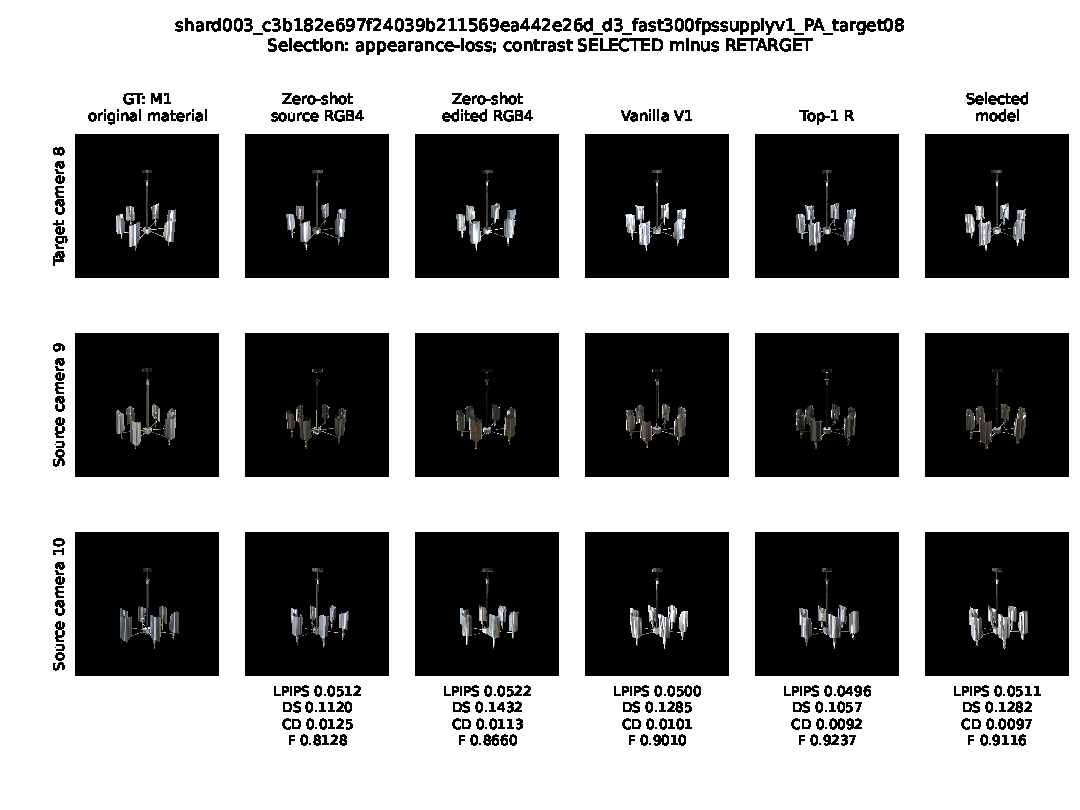
\includegraphics[width=\textwidth]{final-results/figures/example-05.pdf}
\caption{Actual scored frozen TEST example. Rows are target8/source9/source10; columns are the common original-material M1 reference and every frozen model. Selection: appearance-loss. Full-frame panels use the scored archive and official uint8 conversion, without model-specific crop, alignment or rerender. Source annotations use cameras9/10. Conditional categories illustrate their stated conditions and do not estimate population success rates.}
\label{fig:final-qualitative-05}
\end{figure*}

\fi

\subsection{Execution and reproducibility scope}
All 5 fixed pipelines use 508 test examples from 134 source clusters and one
prescribed generation noise per example. Global occupancy ratios are
distinguished from mean per-asset IoU. All 2,540 SS archives are checked for
actual latent hashes, packed occupancy and TP/FP/FN consistency; occupancy is
not substituted for surface CD/F-Score or appearance metrics. Generated
geometry is not aligned independently per output. PBR comparisons retaining
the same geometry use identical original guide values/order/scale and
rendering triangles.

The test campaign bounds complete-asset credits and retires only local raw
duplicates after every declared consumer completes and fresh canonical
file-server SHA/size checks pass. Scored images, guides, reports, source
assets and weights are retained. An initial storage-connection metadata
omission caused a controlled stop; the recovered namespace retains the same
frozen model/numerical protocol and SS inputs. Operational reader-ledger
transactions are serialized without signalling GPU workers. Such recovery
does not constitute a new model or a test-driven hyperparameter choice.
The final metric and qualitative artifacts retain actual producer/file hashes
and the original model-freeze/declaration lineage.

\end{document}
